% !TEX root = main.tex

\section{多元函数的积分}
\subsection{重积分基本定义}
\begin{definition}[二重积分]
设$D$是平面上可求面积的有界闭区域,$f(x,y)$定义在$D$上,用任意曲线网将$D$分成有限个可求面积的区域$\Delta\sigma_1,\Delta\sigma_2,\ldots,\Delta\sigma_n$(称为$D$的一个分法),任取$(\xi_i,\eta_i)\in\Delta\sigma_i$,作和
\[\sigma=\sum_{i=1}^nf(\xi_i,\eta_i)\Delta\sigma_i\]
记$d_i$为$\Delta_i$的直径,$\lambda=\max_{1\leq i\leq n}\{d_i\}$,若当$\lambda\to 0$时,$\sigma$的极限存在,则称$f(x,y)$在$D$可积,并称极限值为$f(x,y)$在$D$的二重积分,记为
\[\iint_Df(P)\diff\sigma\text{或}\iint_Df(x,y)\diff x\diff y\]
也即
\[\iint_Df(x,y)\diff x\diff y=\iint_Df(P)\diff\sigma=\lim_{\lambda\to 0}\sum_{i=1}^nf(\xi_i,\eta_i)\Delta\sigma_i\]
\end{definition}
二重积分的基本性质与一元定积分类似(见\ref{sub:riemann}节),在此不再赘述.
\begin{theorem}[富比尼(Fubini)定理]
若$f(x,y)$在矩形区域$D=[a,b]\times[c,d]$可积,且对$[a,b]$上任意$x$,含参变量积分
\[A(x)=\intabu{c}{d}{f(x,y)}{y}\]
存在,则
\[\iint_Df(x,y)\diff x\diff y=\intab{a}{b}{}\intabu{c}{d}{f(x,y)}{y}\]
若$f(x,y)$在$D$上连续,则积分次序可交换.
若$D=\{(x,y)\mid y_1(x)\leq y\leq y_2(x),a\leq x\leq b\}$,$y_1(x),y_2(x)$在$[a,b]$连续,$f(x,y)$在$D$上连续,则
\[\iint_Df(x,y)\diff x\diff y=\intab{a}{b}{}\intabu{y_2(x)}{y_1(x)}{f(x,y)}{y}\]
\end{theorem}
对于三重积分的情况可以这样考虑
\begin{enumerate}
	\item 横向(平面)累加后再纵向加(注意$D_z$是变化的)
	\[\iiint_Vf(x,y,z)\diff x\diff y\diff z=\int_e^f\diff z\iint_{D_z}f(x,y,z)\diff x\diff y\]
	\item 纵向累加后再横向加(即投影到$D$上)
	\[\iiint_Vf(x,y,z)\diff x\diff y\diff z=\iint_D\diff x\diff y\int_{x_1(x,y)}^{x_2(x,y)}f(x,y,z)\diff z\]
\end{enumerate}
二重积分的几何直观是曲顶柱体的体积,或者是平面薄片的质量.
而三重积分则是四维空间曲顶柱体的提及,或者是空间物体的质量.

\subsection{重积分的变量代换}
\begin{theorem}
设变换
\[T:\begin{cases}x=\varphi(u,v)\\y=\psi(u,v)\end{cases}\]
把$Ouv$平面上由逐段光滑的闭曲线围成的区域$\Delta$一一映射为$Oxy$平面的区域$D$,且$\varphi,\psi$在$\Delta$有二阶连续偏导数,
\[J(u,v)=\frac{\partial(x,y)}{\partial(u,v)}\ne 0,\,(u,v)\in\Delta\]
而$f(x,y)$是定义在$D$上的连续函数,则
\[\iint_Df(x,y)\diff x\diff y=\iint_\Delta f(\varphi(u,v),\psi(u,v))|J(u,v)|\diff u\diff v\]
用微元的观点看,即
\[\diff S=|J(u,v)|\diff\sigma\]
\end{theorem}
用微元的观点看会简单很多,关键确定好变换后的积分区间.
\par 三种常见的积分变换如下
\begin{enumerate}
	\item 极坐标
	\[\begin{cases}x=r\cos\theta\\y=r\sin\theta\end{cases}\implies J(r,\theta)=\frac{\partial(x,y)}{\partial(r,\theta)}=\vmat{\cos\theta & -r\sin\theta\\\sin\theta & r\cos\theta}=r\]
	\item 柱坐标变换
	\[\begin{cases}x=r\cos\theta\\y=r\sin\theta\\z=z\end{cases}\implies J(r,\theta,z)=\frac{\partial(x,y,z)}{\partial(r,\theta,z)}=\vmat{\cos\theta & -r\sin\theta & 0\\\sin\theta & r\cos\theta & 0\\ 0 & 0 & 1}=r\]
	\item 球坐标变换
	\[\begin{cases}x=r\cos\theta\sin\varphi&0\leq<+\infty\\y=r\sin\theta\sin\varphi&0\leq\theta<2\pi\\z=r\cos\varphi & 0\leq\varphi\leq\pi\end{cases}\implies J(r,\theta,\varphi)=\vmat{\cos\theta\sin\varphi & -r\sin\theta\sin\varphi & r\cos\theta\cos\varphi\\\sin\theta\sin\varphi & r\cos\theta\sin\varphi & r\sin\theta\cos\varphi\\ \cos\varphi & 0 & -r\sin\varphi}=-r^2\sin\varphi\]
\end{enumerate}

\subsection{曲线积分}
\subsubsection{第一型曲线及曲面积分}
\begin{definition}[第一型曲线积分]
设$L$为空间可求长的曲线段,$f(x,y,z)$定义在$L$上,$L$的两端点为$A,B$,依次用分点$A=A_0,A_1,\ldots,A_n=B$将$L$分为$n$小段,每小段的弧长记为$\Delta s_i$,不妨将第$i$段小弧也记为$\Delta s_i$,任取$(\xi_i,\eta_i,\zeta_i)\in\Delta s_i$,作和式
\[\sum_{i=1}^n f(\xi_i,\eta_i,\zeta_i)\Delta s_i\]
若当$\lambda=\max_{1\leq i\leq n}\{\Delta s_i\}\to 0$时上述和式极限存在,则称此极限值为$f(x,y,z)$在曲线$L$上的第一型曲线积分,记为
\[\int_Lf(x,y,z)\diff s=\lim_{\lambda\to 0}\sum_{i=1}^nf(\xi_i,\eta_i,\zeta_i)\Delta s_i\]
若$L$为光滑曲线
\[x=x(t),y=y(t),z=z(t),\alpha\leq t\leq\beta\]
$f(x,y,z)$在$L$上连续,则$f(x,y,z)$在$L$上的第一型曲线积分存在,有
\[\int_Lf(x,y,z)\diff s=\intabu{\alpha}{\beta}{f(x(t),y(t),z(t))\sqrt{{x'}^2(t)+{y'}^2(t)+{z'}^2(t)}}{t}\]
\end{definition}
由于第一型曲线积分是无向的,故
\[\int_{\wideparen{AB}}f(x,y,z)\diff s=\int_{\wideparen{BA}}f(x,y,z)\diff s\]
\begin{definition}[第一型曲面积分]
设$S$是空间光滑曲面$z=z(x,y),(x,y)\in D$,$f(x,y,z)$是定义在$S$上的函数,对于$D$的任意分法$\Delta\sigma_i$,相应地得到$S$的分法$\Delta S_i$,任取$(\xi_i,\eta_i,\zeta_i)\in\Delta S_i$,记$\lambda=\max_{1\leq i\leq n}\{d(\Delta\sigma_i)\}$,则第一型曲面积分记为
\[\iint_S f(x,y,z)\diff S=\lim_{\lambda\to 0}\sum_{i=1}^n f(\xi_i,\eta_i,\zeta_i)\Delta S_i\]
若$D$为有界闭区域,$f(x,y,z)$在$S$上连续,则$f(x,y,z)$在曲面$S$上的第一型曲面积分存在,且
\[\iint_S f(x,y,z)\diff S=\iint_D f(x,y,z(x,y))\sqrt{1+z_x^2(x,y)+z_y^2(x,y)}\diff x\diff y\]
\end{definition}
求第一型曲面积分,关键是将曲面投影到$xOy$平面上(即$D$),即可将曲面积分变为二重积分.

\subsubsection{第二型曲线积分及曲面积分}
\begin{definition}[第二型曲线积分]
设向量函数$\vF(x,y,z)=P(x,y,z)\vi+Q(x,y,z)\vj+R(x,y,z)\vk$定义在空间光滑曲线弧$L$上,则
\[\begin{aligned}
\int_L\vF(x,y,z)\cdot\diff\vs&=\int_LP(x,y,z)\diff x+Q(x,y,z)\diff y+R(x,y,z)\diff z\\
&=\lim_{\lambda\to 0}\sum_{i=1}^n[P(\xi_i,\eta_i,\zeta_i)\Delta x_i+Q(\xi_i,\eta_i,\zeta_i)\Delta y_i+R(\xi_i,\eta_i,\zeta_i)\Delta z_i]
\end{aligned}\]
\end{definition}
若$L$为闭曲线,则记
\[\oint_LP\diff x+Q\diff y+R\diff z\]
此时积分与起点选择无关,只与曲线$L$的方向有关.
\par 注意积分公式中定积分的下限总是对应有向曲线段的起点,上限总是对应有线曲线段的终点.
路径不同,积分值可能不同.
\[\int_{\wideparen{AB}}\vF\cdot \diff\vs=\int_{\arc{AB}}\vF\cdot\vtau\diff d\]
其中,$\vtau$是与$\arc{AB}$方向一致的单位切向量
用分量表示即为
\[(\diff x,\diff y,\diff z)=(\cos\alpha,\cos\beta,\cos\gamma)=(\frac{\diff x}{\diff s},\frac{\diff y}{\diff s},\frac{\diff z}{\diff s})\]
\begin{definition}[第二型曲面积分]
\[\begin{aligned}
\iint_S\vF(x,y,z)\cdot\diff\vS&=\iint_SP(x,y,z)\diff y\diff z+Q(x,y,z)\diff z\diff x+R(x,y,z)\diff x\diff y\\
&=\iint_S(P\cos\alpha+Q\cos\beta+R\cos\gamma)\diff S
\end{aligned}\]
这里的$(\cos\alpha,\cos\beta,\cos\gamma)$是法向量与坐标轴的夹角
\end{definition}

\subsubsection{各类积分之间的联系}
\begin{definition}[连通区域]
平面区域$D$上任何一条封闭曲线都可以不经过$D$以外的点而连续地收缩为属于$D$的一点,则称$D$为平面单连通区域,否则为复连通区域
\end{definition}
\begin{center}
\begin{tabular}{|c|c|c|}\hline
第一型曲线积分(一线) & $\disp\int_\mL f(x,y,z)\diff l$ & 线密度\\\hline
第二型曲线积分(二线) & $\disp\int_\mL\vF(x,y,z)\cdot\diff\vl$ & 变力做功\\\hline
第一型曲面积分(一面) & $\disp\iint_\mS f(x,y,z)\diff S$ & 面密度\\\hline
第二型曲面积分(二面) & $\disp\iint_\mS\vF(x,y,z)\cdot\diff\vS$ & 流量\\\hline
\end{tabular}
\end{center}
\par 牛顿-莱布尼茨公式在高维空间的推广,即将内部积分转化为边界积分
\begin{theorem}[格林(Green)公式]
\[\iint_D\pd{P}{y}-\pd{Q}{x}\diff x\diff y=\iint_D\vmat{\pd{}{x}&\pd{}{y}\\P&Q}=\oint_LP\diff x+Q\diff y\]
\end{theorem}
平面区域$D$的面积
\[|D|=\iint_D\diff x\diff y=\frac{1}{2}\oint_Lx\diff y-y\diff x\]
\begin{theorem}[高斯(Gauss)公式]
\[\iiint_V\lrp{\pd{P}{x}+\pd{Q}{y}+\pd{R}{z}}\diff x\diff y\diff z=\oiint_SP\diff y\diff z+Q\diff z\diff x+R\diff x\diff y\]
$S$方向为外侧
\end{theorem}
\begin{theorem}[斯托克斯(Stokes)公式]
\[\begin{aligned}
\oint_\mL P\diff x+Q\diff y+R\diff z&=\oint_\mL\lrp{\pd{R}{y}-\pd{Q}{z}}\diff y\diff z+\lrp{\pd{P}{z}-\pd{R}{x}}\diff z\diff x+\lrp{\pd{Q}{x}-\pd{P}{y}}\diff x\diff y\\
&=\iint_S\vmat{\diff y\diff z&\diff z\diff x&\diff x\diff y\\\pd{}{x}&\pd{}{y}&\pd{}{z}\\P&Q&R}\\
&=\iint_S\vmat{\cos\alpha&\cos\beta&\cos\gamma\\\pd{}{x}&\pd{}{y}&\pd{}{z}\\P&Q&R}\diff S
\end{aligned}\]
\end{theorem}

结合场论的符号(见第\ref{sec:field}章),可以得到以下这张关系图.
其中,$\vtau$是与$\mL$方向一致的\textbf{单位切向量},$\vn$是与$\mS$同侧的\textbf{单位法向量},且有
\[\begin{aligned}
\diff\vl&=\vtau\diff l=(\cos(\vtau,x),\cos(\vtau,y),\cos(\vtau,z))\diff l=(\diff x,\diff y,\diff z)\\
\diff\vS&=\vn\diff S=(\cos(\vn,x),\cos(\vn,y),\cos(\vn,z))\diff S=(\diff y\diff z,\diff z\diff x,\diff x\diff y)
\end{aligned}\]
\begin{figure}[H]
\centering
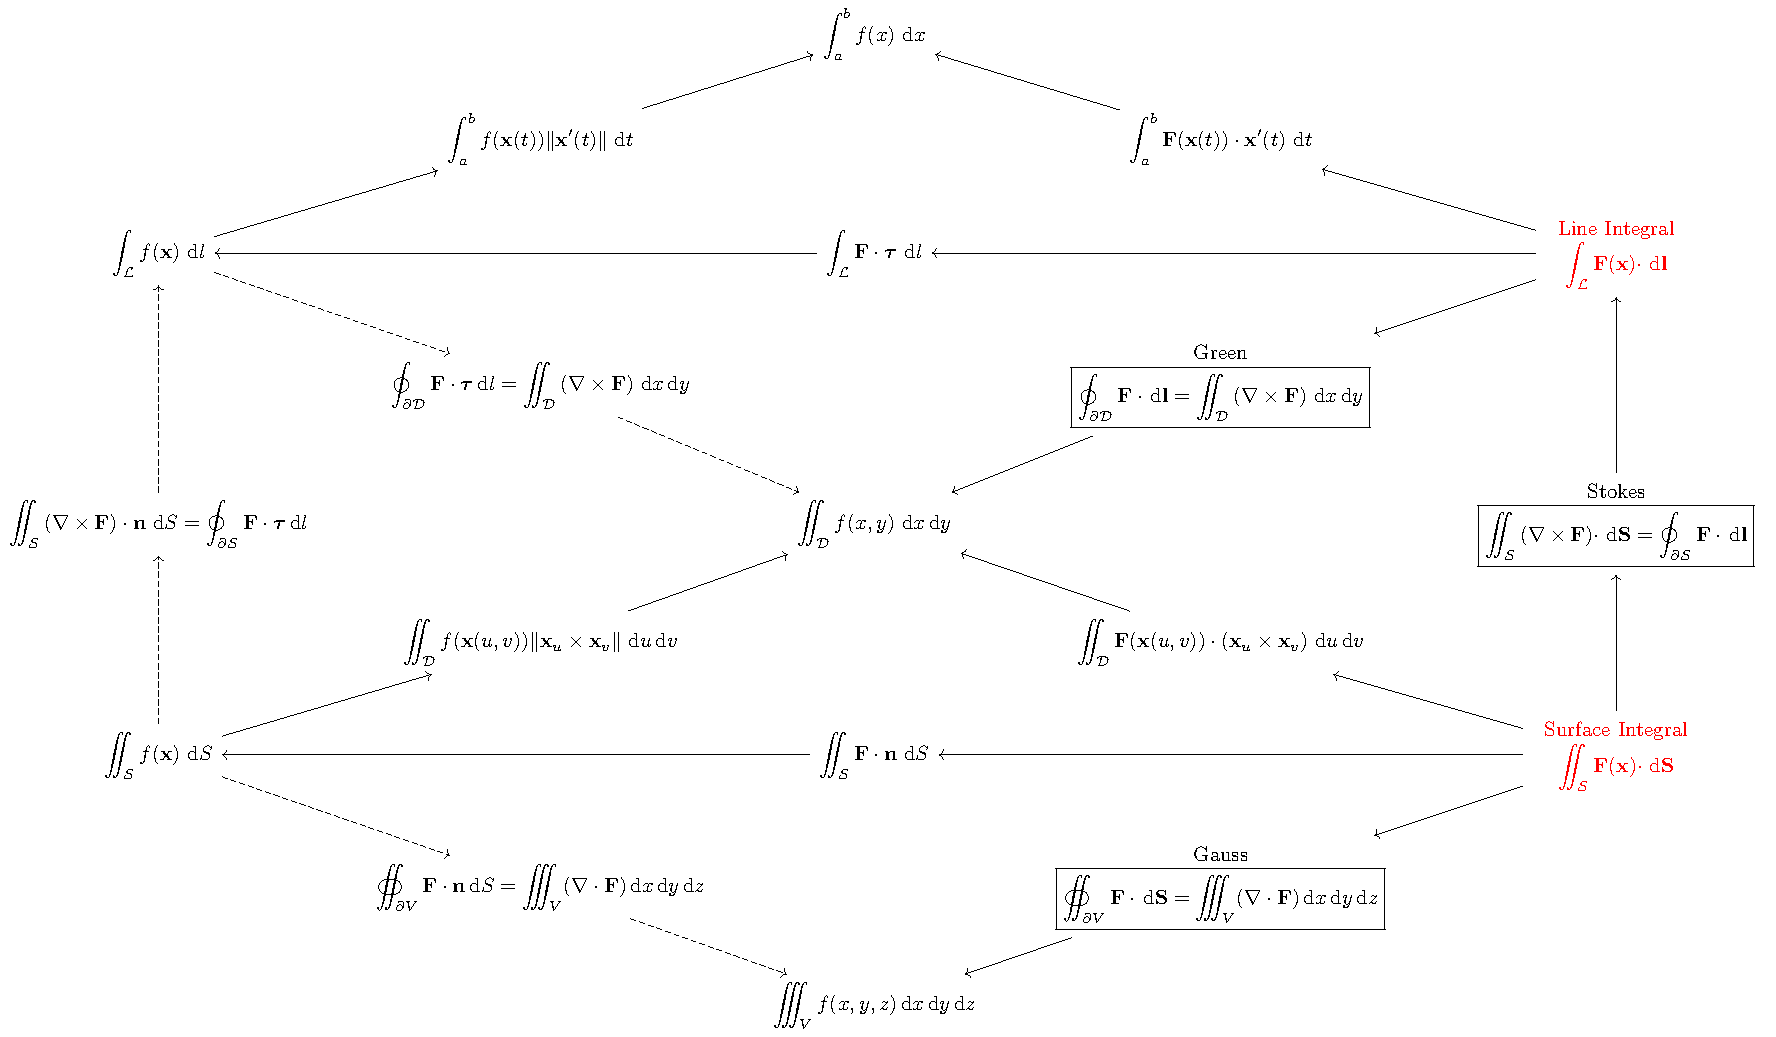
\includegraphics[width=\linewidth]{fig/multivar-integral-relationship.pdf}
\end{figure}
\par 三大公式用外微分形式表示,如$\partial\mD$表示$\mD$区域的边界.
\par 同时注意
\[\vx_u\times\vx_v=\lrp{\pd{(u,v)}{(y,z)},\pd{(u,v)}{(z,x)},\pd{(u,v)}{(x,y)}}\]

\subsubsection{积分与路径无关}
\begin{theorem}
设$D$为平面单连通区域,函数$P(x,y)$,$Q(x,y)$在$D$上有连续偏导数,则下列四个命题等价
\begin{enumerate}
	\item 沿$D$中任一逐段光滑闭曲线$L$,有
	\[\oint_LP\diff x+Q\diff y=0\]
	\item 对$D$中任一逐段光滑曲线$L$,曲线积分
	\[\int_LP\diff x+Q\diff y\]
	与路径无关,只与$L$的起点和终点有关
	\item 微分式$P\diff x+Q\diff y$在$D$内是某函数$u(x,y)$的全微分,即有
	\[\diff u=P\diff x+Q\diff y\]
	\item 在$D$内每一点有
	\[\vmat{\vi&\vj\\\pd{P}{y}&\pd{Q}{x}}=0\]
\end{enumerate}
\end{theorem}
\begin{theorem}[奇点]
关于奇点的结论
\begin{enumerate}
	\item 对$D$内任意一条不包围奇点的闭曲线$L$,有
	\[\oint_LP\diff x+Q\diff y=0\]
	\item 环绕某一奇点的任意两条简单闭曲线$L_1,L_2$的积分相等,即
	\[\oint_{L_1}P\diff x+Q\diff y=\oint_{L_2}P\diff x+Q\diff y\]
	这个公共值称为该奇点的循环常数
\end{enumerate}
\end{theorem}